\section{Parameter Sweep}
\label{param_sweep_section}

In order to find the parameters for the two enhanced models that maximise some of our scores, we run a full parameter sweep on a subset of the samples with two parameters related to training.
\begin{table}[h]
	\centering
	\begin{tabular}{r | l l l}
		\toprule
			Parameter & \multicolumn{3}{|c}{Values} \\
		\midrule
			Learning Rate ($\alpha$) & 0.01 & 0.001 & 0.0001 \\
			Cosine Similarity Weight ($\varkappa$) & 0 & 0.2 & 0.5 \\
		\bottomrule
	\end{tabular}
\end{table}

Each model is run for 15 epochs, since in our experiments that's enough for finding a trend in the metrics, and is judged in three of the metrics presented in \cref{scoring_section}: F1-score of Rouge1, F1-score of Rouge2, and cosine similarity score.

\subsection{Transformer Model}

The results can be found in the three scatter plots in \cref{sweep_results}.
\begin{figure}[h]
	\centering
	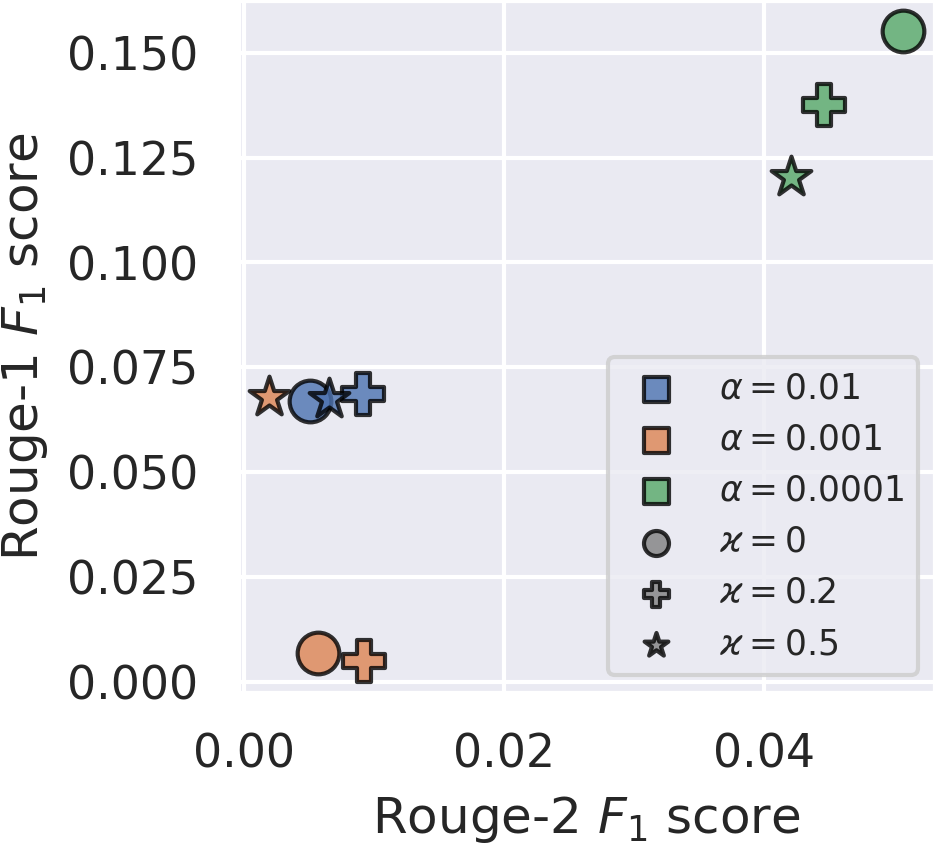
\includegraphics[width=.32\textwidth]{sweep_rouge1_v_rouge2.png} \hfill{}
	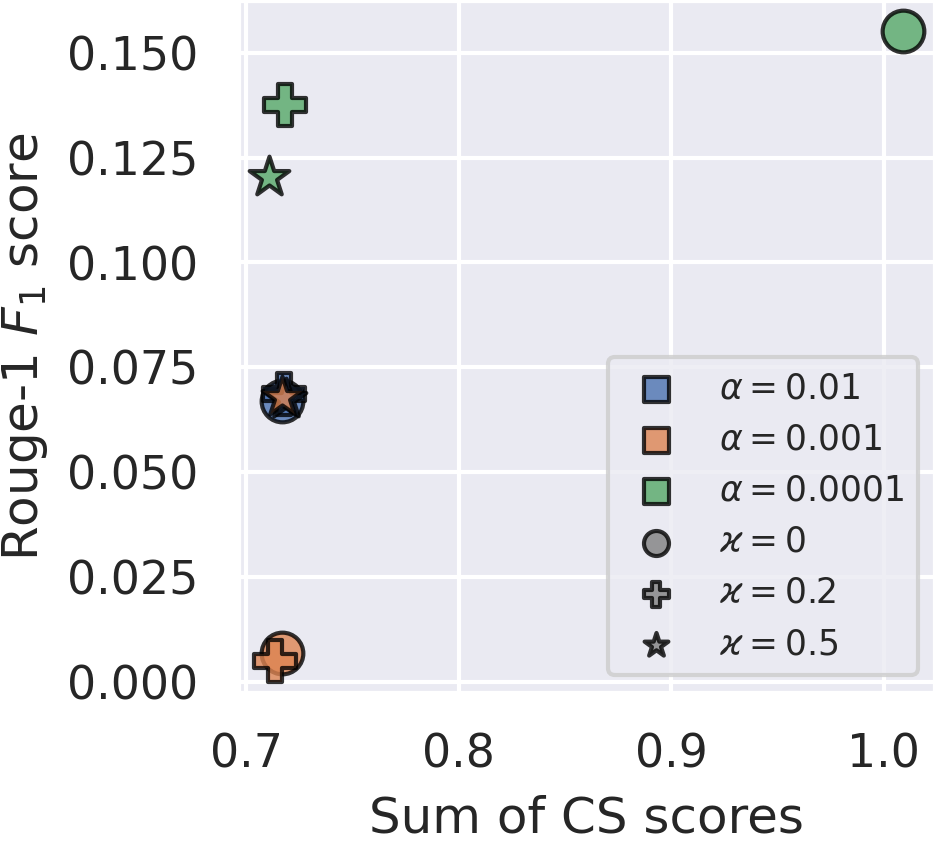
\includegraphics[width=.32\textwidth]{sweep_rouge1_v_cs.png} \hfill{}
	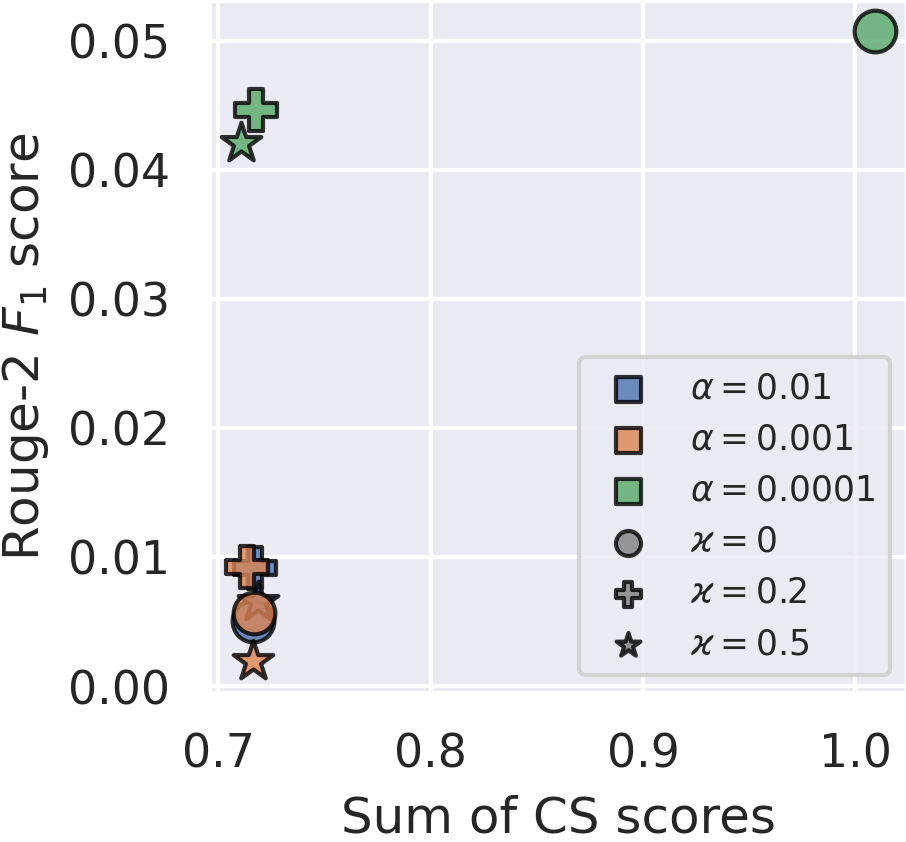
\includegraphics[width=.32\textwidth]{sweep_rouge2_v_cs.png}
	\caption{Results of parameter sweep of the transformer for different $\alpha$ and $\varkappa$ values. For all three scores, $\alpha = 0.0001$ and $\varkappa = 0$ presents the best results.}
	\label{sweep_results}
\end{figure}

The main results from the parameter sweep clearly demonstrate that, in the case of this transformer, a low learning rate produces better results in all metrics that a high learning rate.
This is a bit surprising given the large amount of parameters the transformer, but it's likely related to how unstable problem in sequence analysis are: even a small change in weights produces a large change in these metrics, so convergence must be slower.

Additionally, it's sadly clear that the best result at this learning rate happen when $\varkappa = 0$.
While using cosine similarity loss as a fraction of the final loss seemed like a fine idea, it's likely that it adds extra instability to the gradient descent.

\subsection{BERTFormer}

The results from the parameter sweep can be found in the three scatter plots in \cref{bertformer_sweep_results}.

\begin{figure}[h]
	\centering
	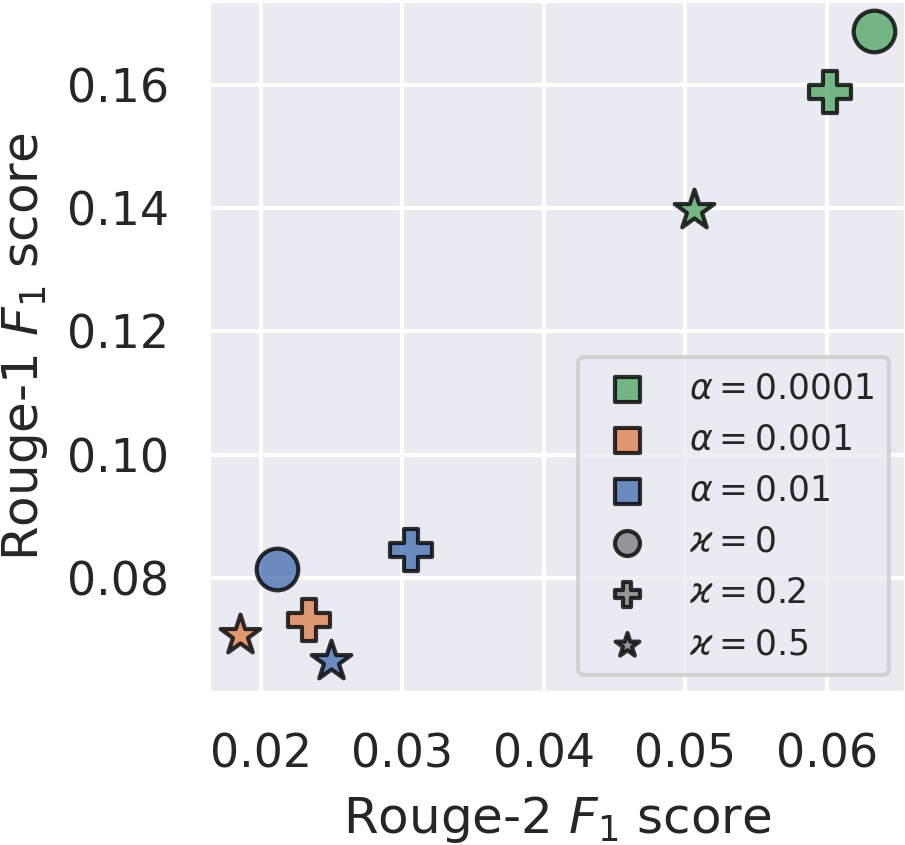
\includegraphics[width=.32\textwidth]{bertformer_sweep_rouge1_v_rouge2.png} \hfill{}
	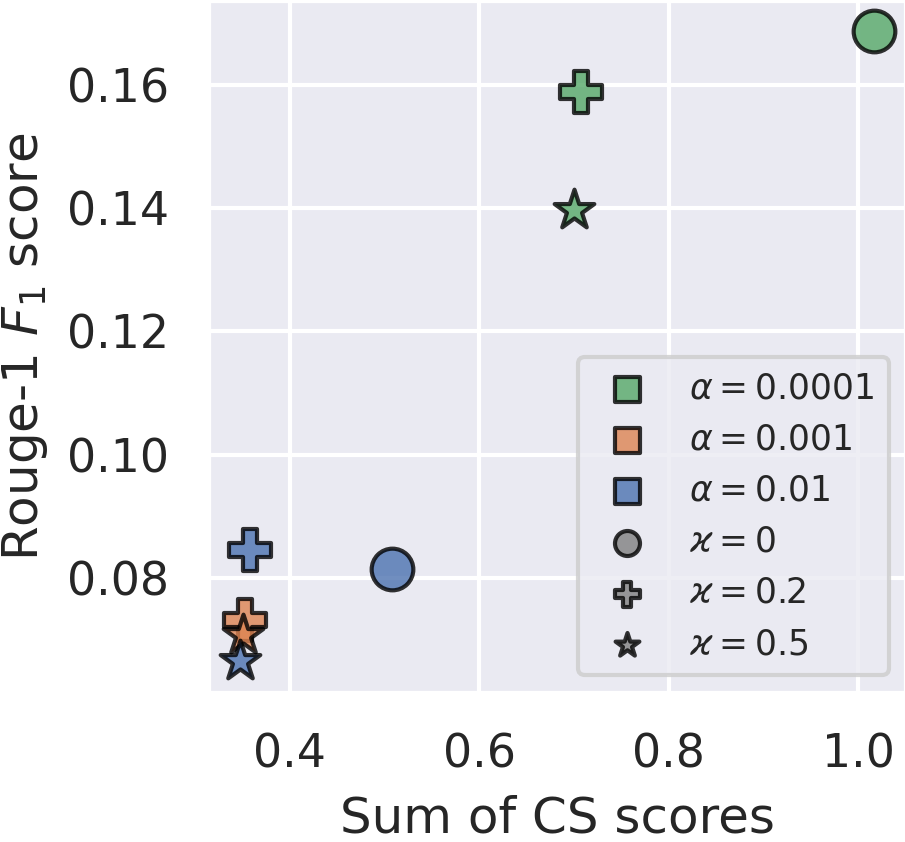
\includegraphics[width=.32\textwidth]{bertformer_sweep_rouge1_v_cs.png} \hfill{}
	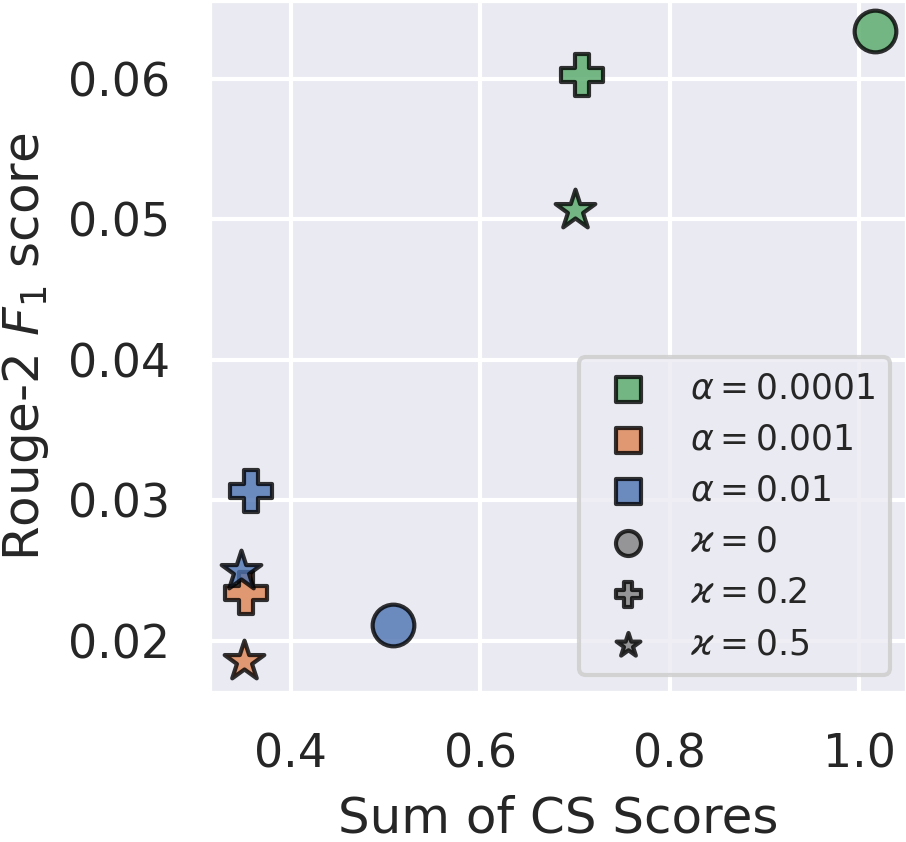
\includegraphics[width=.32\textwidth]{bertformer_sweep_rouge2_v_cs.png}
	\caption{Results of parameter sweep of the transformer for different $\alpha$ and $\varkappa$ values. For all three scores, $\alpha = 0.0001$ and $\varkappa = 0$ presents the best results.}
	\label{bertformer_sweep_results}
	\vspace{-7pt}
\end{figure}

The results are very similar to those in \cref{sweep_results}, and both parameter sweeps have a clear winner with low learning rate and no use of cosine similarity loss ($\varpappa = 0$).

Despite this, the BERTFormer models using $\varkappa > 0$ seems to have better results on CS score than the Transformer model when trained on the small amount of samples that were needed for a run in this parameter sweep.
This is likely due to the pre-trained encoder producing more sensible language without need for much training, and is worth experiment on in the future.

\subsection{Final Results}

\begin{table}[h]
	\centering
	\begin{tabular}{l c | c c | c c c}
		\toprule
			Model & Best & $\alpha$ & $\varkappa$ & Rouge-1 $F_1$ & Rouge-2 $F_1$ & Sum of CS \\
		\midrule
			Transformer & 
\includegraphics[width=9pt,height=9pt]{green_circle.png} & 0.0001 & 0 & 0.17 & 0.69 & 1.02 \\
			BERTFormer & 
\includegraphics[width=9pt,height=9pt]{green_circle.png} & 0.0001 & 0 & 0.16 & 0.62 & 1.01 \\
		\bottomrule
	\end{tabular}
	\caption{The models with the best scores in the hyperparameter, which contains the parameters we will use for them from now on.}
\end{table}

